\part{Analysis}

A hand digit recognition neural network (HDR-NN) model is implementated in C, C++ Eigen, Python Numpy and Pytorch. The performance of HDR-NN training implementations was evaluated on the iMX6SDB evaluation board, which was programmed with an Embedded Linux built using The Yocto Project. To gauge the effectiveness of the models, we compared model accuracy, execution time, and peak memory usage while altering the number of layers and neurons in each layer. The results of these measurements are presented in the following chapters along with discussions on the obstacles encountered in developing the NN model and compiling it to operate on the target hardware.

%Ideas: 1. Coefficient of variation
%		2. optimisation flags
%		3. Measurements using different tools
%		4. Early stopping
%		5. Choosing Model parameters
%		6. Extrapolation

\chapter{Measurement}

The benchmark applications were executed on an embedded linux operating system and the measurements were taken primarily based on the \textit{times} system call and perf\_events linux API. The primary tools for current measurement values given in the following chapter were taken using the GNU time. GNU Time provides timing statistics such as the elapsed real time between invocation and termination, the user CPU time, and the system CPU time, the later two via the \textit{times} system call API. GNU Time also provides output lots of useful information on other resources like memory, I/O and IPC calls where available.

The priliminary measurements for the different executions completed with different learning algorithm parameters and model shapes across implementations were timing statistics and maximum resident set size (alternatively refered to as peak memory utilisation in the following chapter)

\section{Benchmark Application Parameters}

\chapter{Results}
A hand digit recognition application is implemented in different paradigms, specifically C, C++, Python, and Pytorch, which are the benchmark applications. Each this application is a fully connected feedforward neural network composed of multiple layers of neurons connected in a directed graph. The model has a constant input size of 784 and output size of 10. The hidden layer sizes vary depending on the implementation:
\begin{itemize}
	\item C and C++ Eigen: 2, 4, 8, 32, 128, (32,16), and (128,16)
	\item Python-Numpy: 2, 8, 32, (32,16)
	\item Tensorflow/Pytorch:
\end{itemize}
The MNIST dataset is selected to train the model. This dataset contains 60,000 training images and 10,000 test images of hand-written digits. The model is trained using stochastic gradient descent, which is an optimization algorithm used to minimize a loss function. The backpropagation algorithm is used to calculate the gradients of the loss function with respect to the weights of the network. Finally, the mean square error loss function is used to measure the difference between the predicted output and the actual output of the network. The values of the biases and weights are initialized randomly with the PNGR random generator and a starting seed which are chosen to be identical for the different benchmark applications. The training hyperparameters are set to 30 epochs with a batch size of 10, a learning rate of 3 and sigmoid activation.

It is essential that the hardware utilsed for benchmarking closely resembles the Scania ECU's IMX6 processor, as this will make it easier to replicate the experiment on a repurposed ECU and will also provide the most precise results. The IMX6Q-SABRE Smart Devices evaluation board, which is armed with four 32-bit Cortex A9 cores, is an ideal choice. The Cortex A9 core is equipped with ARM V7 instruction set architecture and a powerful VFPv3 floating point unit with NEON SIMD capabilities. The processor has 32 KB instruction and data L1 caches, 1 MB L2 cache and 1 GB DDR3 SDRAM memory. The benchmark applications are designed to be run on a single core of the IMX6 processor, although it supports quad-core, to ensure the experiment is straightforward and easier to manage. This will also guarantee that the results are precise and accurate.

The yocto project is used to create a custom embedded linux distribution for the imx6qsabresd machine. The NXP yocto project guide (link) provides the instructions for building the Linux image, and additional packages such as cmake, python3 are installed during the build. The resulting image file, which used to flash the hardware, has a size of ~300Mb.

The accuracy of the model is evaluated after each training epoch on the MNIST test set. After the training of the model for 30 epochs, the final weights and biases of the network and the accuracy on the test set are saved for analysis. This data is used to verify the correctness of the NN model in each benchmark application.
The GNU time program is a great tool for monitoring the performance of applications. It allows us to measure the execution time and peak memory usage, which is used to compare the effectiveness of training the neural network model on the custom hardware implemented with different paradigms.

The python script created runs the experiment, executing each of the benchmark applications (C, C++, Python, Pytorch) one after the other. Every benchmark application is designed to be repeated 10 times, and all the measurements for each of the hidden layer configurations are saved for each of these iterations. The average values of the model accuracy, execution time and peak memory usage across all iterations are utilized for the analysis.

(we also reason the impact of execution time in the decision to skip some network configurations and add a table of the experiments conducted)


\section{Evaluating Correctness}
\subsection{Accuracy}
The different implementation perform similarly in model accuracy. This is expected as the models have the exact structure and configurations.
\begin{figure}[ht]
	\centering
	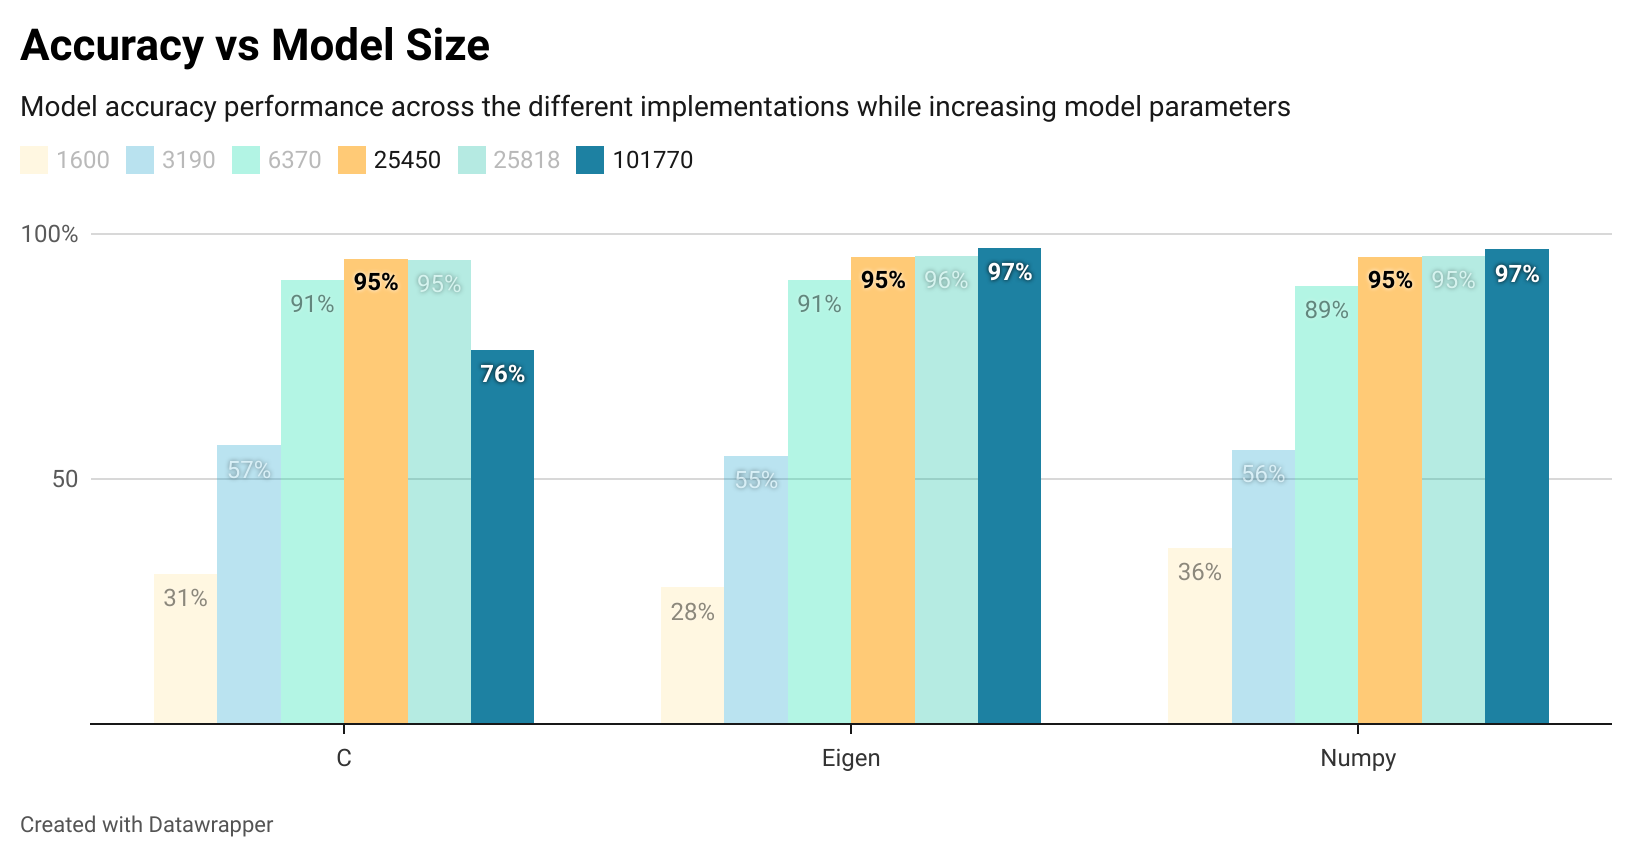
\includegraphics[scale=0.37]{accuracy}
	\caption[HDR-NN Accuracy]{Comparing the accuracy of the different HDR-NN implementations.}
\end{figure}
Further, when the number of neurons in a single layer exceeds 32, the accuracy of the C implementation is observed to decrease due to (a bug). To improve accuracy, adding another layer with 16 neurons is found to be beneficial without significantly increasing the time required for computation. In fact, for larger network sizes, it is observed to even reduce the computation time required. (separate plot for this behaviour)

(Here, we also evaluate the error in accuray and plot it for each network configuration)

\subsection{Weights and Biases}
Here, we evaluate the approximation error in the generated weights and biases between the different implementation. Also, we reason how the data structure in each of the implementation influence the error.


\section{Evaluating effectiveness}
\subsection{Execution Time}
The training time of the neural network applications increases exponentially as the network size increases by the power of 2 because the number of parameters in a fully connected network increases exponentially as the number of neurons increases. This leads to an increase in the amount of calculations needed for the network to learn, resulting in a longer run time for the training process.

\begin{figure}[ht]
	\centering
	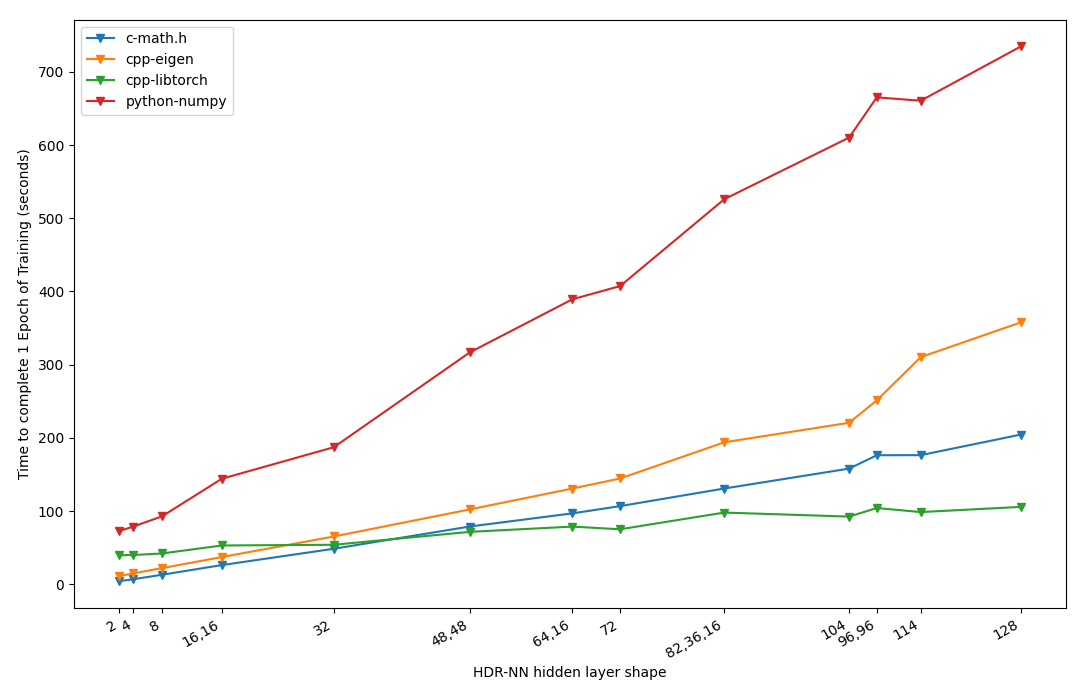
\includegraphics[scale=0.32]{exec-time}
	\caption[Execution Time vs Model Parameters]{Comparing total run time for training the different HDR-NN programs}
\end{figure}

(here we evaluate the percentage/ratio/Coefficient of variation (cov) between the applications.)

\subsection{Peak Memory Usage}
Regardless of the hidden layer sizes, the peak memory utilisation remains constant for the NN application across all implementations. The C++ Eigen implementation has the lowest run time memory footprint, while Python Numpy is the least efficient.

\begin{figure}[ht]
	\centering
	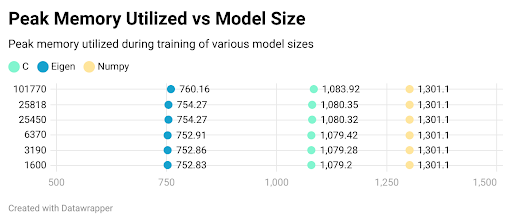
\includegraphics[scale=0.30]{memory-bar}
	\caption[Peak Memory Utilisation]{Peak Memory Utilized during training with different model sizes remain similar within the same implementation}
\end{figure}

(here we evaluate the percentage/ratio/cov between the applications.)

\subsection{Profiling}

\subsection{Failure/Fault testing}

\chapter{Discussion}

% \section{Coefficient of variation}
% A total of 10 iterations were conducted to ensure that the results remained consistent. To assess the degree of variability among the various trials, the mean and standard deviation were calculated across all runs, and their ratio was determined. This ratio indicates the level of variation between the different tests.

\section{Developer Experience}

\section{Early stopping}
The training for all the implementations were executed by configuring the number of epochs as 30. This leads to the accuracy of model dropping significantly due to overfitting, which could be avoided if early stopping was implemented.
But, early stopping is not implemented as the performance would be completely different and there wouldn't be a standard setting to compare the implementations.

\section{General Distribution of Work}

\chapter{Conclusion and Future Work}
\textit{What does it all mean? Where do we go from here?}
